%! Unidad 3 — Óptica geométrica (teoría, actividades resueltas y prácticas)
%! Fuente: Fuentes/Tema_3.pdf (reescrito; datos de las actividades cambiados y recalculados)

\section*{Para empezar: la cámara oscura}
\addcontentsline{toc}{section}{Para empezar: la cámara oscura}

Si en una habitación completamente a oscuras se abre un agujero pequeño en la persiana, en la pared de enfrente aparece
la imagen de la calle, con sus colores y su movimiento\ldots{} pero cabeza abajo. Ya lo describieron Aristóteles y el
científico árabe Alhacén, y los pintores del Renacimiento lo usaban para copiar paisajes. Para explicarlo basta una idea:
\emph{la luz viaja en línea recta}. Los rayos que salen de lo alto de un árbol pasan por el agujero y llegan a la parte baja
de la pared, y al revés. En esta unidad usaremos esa idea, la del rayo de luz, para entender cómo se forman las imágenes en
espejos, lentes, el ojo humano y los instrumentos ópticos: es la \textbf{óptica geométrica}.

\section{La naturaleza de la luz}\label{sec:opt-naturaleza}

La pregunta «¿qué es la luz?» ha tenido respuestas distintas a lo largo de la historia:
\begin{itemize}
    \item \textbf{Modelo corpuscular} (Newton, siglo \textsc{xvii}). La luz está formada por partículas diminutas que
    salen del foco a gran velocidad y viajan en línea recta. Explicaba bien la propagación rectilínea y la reflexión, pero
    tenía problemas con la refracción y no explicaba cómo pueden cruzarse dos haces de luz sin chocar.
    \item \textbf{Modelo ondulatorio} (Huygens, siglo \textsc{xvii}). La luz es una onda. Huygens pensaba que era
    longitudinal, como el sonido, y que necesitaba un medio, el \emph{éter}, para propagarse. Al principio tuvo poco apoyo
    frente a la autoridad de Newton.
    \item \textbf{Triunfo de las ondas} (siglo \textsc{xix}). Young obtuvo interferencias con luz y Fresnel explicó la
    difracción y la polarización suponiendo que la luz es una onda \emph{transversal}. Después, Maxwell demostró que la luz
    es una \textbf{onda electromagnética}, que puede propagarse en el vacío.
    \item \textbf{Dualidad onda-corpúsculo} (siglo \textsc{xx}). Einstein explicó el efecto fotoeléctrico suponiendo que la
    luz está formada por «paquetes» de energía, los \emph{fotones} (lo veremos en la unidad de física cuántica).
\end{itemize}

\begin{remark}
    Hoy se acepta que la luz tiene un \textbf{comportamiento dual}: en la propagación, las interferencias, la difracción o
    la polarización se comporta como una onda; cuando interacciona con la materia (efecto fotoeléctrico, efecto Compton),
    como un chorro de partículas. En un mismo fenómeno nunca muestra los dos comportamientos a la vez.
\end{remark}

\section{Propagación de la luz}\label{sec:opt-propagacion}

\subsection{Propagación rectilínea}\label{subsec:opt-rectilinea}

En un medio homogéneo la luz se propaga en línea recta. Las líneas que indican la dirección de propagación son los
\azuln{rayos}, perpendiculares a los frentes de onda. Según cómo se comportan frente a la luz, los cuerpos pueden ser
\emph{opacos} (no dejan pasar la luz), \emph{transparentes} (la dejan pasar y se ve a través de ellos, como el vidrio) o
\emph{translúcidos} (la dejan pasar, pero no se distinguen los objetos, como el papel vegetal).

La propagación rectilínea explica las \textbf{sombras} y las \textbf{penumbras}: detrás de un cuerpo opaco iluminado por un
foco extenso hay una zona a la que no llega ningún rayo (sombra), otra a la que llegan solo algunos (penumbra) y otra
totalmente iluminada. Los \textbf{eclipses} son el mismo fenómeno a escala astronómica: si la Luna se interpone entre el Sol
y la Tierra, las zonas de la Tierra en su sombra ven un eclipse total de Sol y las que están en la penumbra, uno parcial
(figura~\ref{fig:opt-sombras}).

\begin{figure}[H]
    \centering
    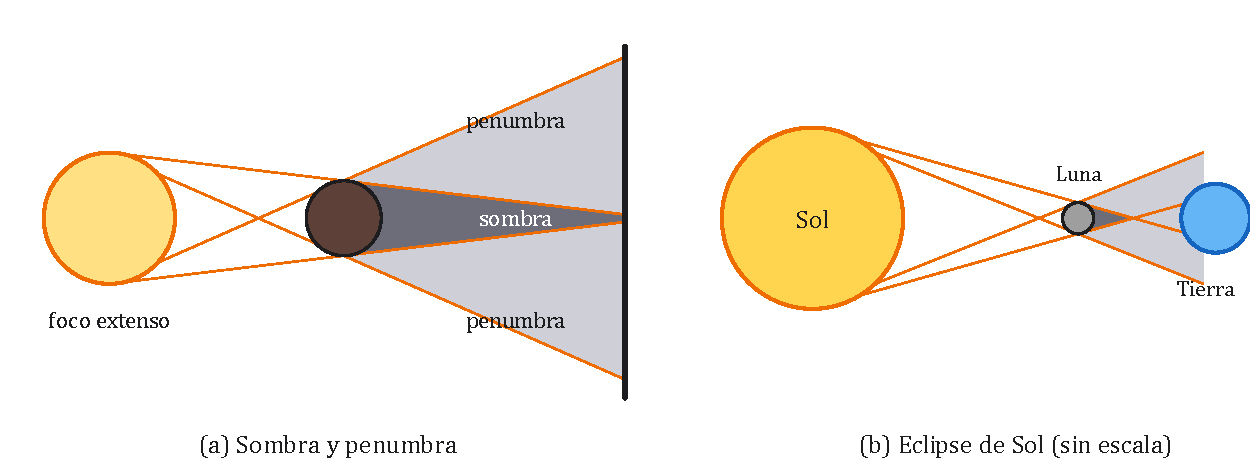
\includegraphics[width=0.95\linewidth]{images/UD3/sombras}
    \caption{(a) Sombra y penumbra de un cuerpo opaco. (b) En un eclipse de Sol la Luna proyecta su sombra sobre la Tierra.}
    \label{fig:opt-sombras}
\end{figure}

\subsection{Velocidad de la luz}\label{subsec:opt-velocidad}

Durante siglos se creyó que la luz se propagaba de forma instantánea. Galileo intentó medir su velocidad con faroles
entre dos colinas, sin éxito. En 1676 el danés Rømer la estimó por primera vez observando los eclipses de las lunas de
Júpiter y obtuvo unos \qty{2.1e8}{\m\per\second}. Fizeau (1849), con una rueda dentada, y Michelson, con espejos giratorios,
mejoraron mucho la medida. Hoy su valor en el vacío está fijado exactamente:
\begin{centeredequation}
    c = \qty{299792458}{\m\per\second} \approx \qty{3e8}{\m\per\second} \label{eq:opt-c}
\end{centeredequation}
En el aire es prácticamente la misma. En los demás medios transparentes la luz va más despacio: en el agua, a unos
\qty{2.25e8}{\m\per\second}, y en el vidrio, a unos \qty{2e8}{\m\per\second}.

\paragraph{El año luz.} En astronomía se usa como unidad de longitud el \azuln{año luz}: la distancia que recorre la luz en
el vacío en un año, \(\qty{1}{\text{a.l.}} = 3\cdot 10^8\cdot 365{,}25\cdot 86400 \approx \qty{9.46e15}{\m}\).

\begin{exercise}
    Cuando Marte está en conjunción, su distancia media al Sol es de unos \qty{2.28e8}{\km}. ¿Cuánto tarda en llegar a Marte
    la luz del Sol?
    \begin{solu}
        \(t = \dfrac{d}{c} = \dfrac{2{,}28\cdot 10^{11}}{3\cdot 10^8} = \textcolor{red}{\qty{760}{\second} \approx \qty{12.7}{\minute}}\).
    \end{solu}
\end{exercise}

\begin{exercise}
    Próxima Centauri, la estrella más cercana al Sol, está a \num{4.24} años luz. ¿A cuántos kilómetros está?
    \begin{solu}
        \(d = 4{,}24\cdot 9{,}46\cdot 10^{12}\ \unit{\km} = \textcolor{red}{\qty{4.01e13}{\km}}\).
    \end{solu}
\end{exercise}

\subsection{Índice de refracción}\label{subsec:opt-indice}

\begin{definition}[Índice de refracción]
    El \rojon{índice de refracción absoluto} de un medio es el cociente entre la velocidad de la luz en el vacío y su
    velocidad en ese medio:
    \begin{centeredequation}
        \boxed{n = \dfrac{c}{v}} \label{eq:opt-indice}
    \end{centeredequation}
    Es adimensional y siempre mayor que 1 (en el vacío, \(n = 1\); en el aire, \(n \approx 1\)).
\end{definition}

Un medio es \azuln{más refringente} que otro si su índice de refracción es mayor: en él la luz va más despacio. Para dos
medios, \(n_1 v_1 = n_2 v_2 = c\), y el \azuln{índice de refracción relativo} del medio 2 respecto del 1 es
\(n_{21} = \dfrac{n_2}{n_1} = \dfrac{v_1}{v_2}\).

\begin{table}[H]
    \centering
    \caption{Índices de refracción de algunas sustancias (luz amarilla)}
    \vspace{-5pt}
    \begin{tabular}{@{}lc@{\hspace{1.5cm}}lc@{}}
        \toprule
        \textbf{Sustancia} & \textbf{\(n\)} & \textbf{Sustancia} & \textbf{\(n\)} \\
        \midrule
        Aire & \num{1.0003} & Vidrio común & \num{1.52} \\[3pt]
        Agua & \num{1.33} & Vidrio \emph{flint} & \num{1.65} \\[3pt]
        Etanol & \num{1.36} & Cuarzo fundido & \num{1.46} \\[3pt]
        Hielo & \num{1.31} & Diamante & \num{2.42} \\
        \bottomrule
    \end{tabular}
    \label{tab:opt-indices}
\end{table}

\paragraph{Frecuencia y longitud de onda.} Al pasar de un medio a otro, la frecuencia de la luz no cambia (la impone el
foco), pero sí su velocidad y, por tanto, su longitud de onda: \(v_1 = \lambda_1\nu\) y \(v_2 = \lambda_2\nu\). Dividiendo:
\begin{centeredequation}
    \dfrac{\lambda_1}{\lambda_2} = \dfrac{v_1}{v_2} = \dfrac{n_2}{n_1} \qquad\Rightarrow\qquad \lambda = \dfrac{\lambda_0}{n} \label{eq:opt-lambda}
\end{centeredequation}
donde \(\lambda_0\) es la longitud de onda en el vacío. El color que percibimos depende de la frecuencia, así que un rayo
rojo sigue siendo rojo dentro del agua.

\begin{exercise}
    Un puntero láser de helio-neón emite luz roja de \qty{633}{\nm} en el vacío. ¿Cuál es su velocidad y su longitud de
    onda dentro del agua (\(n = 1{,}33\))?
    \begin{solu}
        \(v = \dfrac{c}{n} = \dfrac{3\cdot 10^8}{1{,}33} = \textcolor{red}{\qty{2.26e8}{\m\per\second}}\);
        \(\lambda = \dfrac{\lambda_0}{n} = \dfrac{633}{1{,}33} = \textcolor{red}{\qty{476}{\nm}}\).
        \textcolor{blue}{(Sigue viéndose roja: la frecuencia no cambia.)}
    \end{solu}
\end{exercise}

\begin{exercise}
    A veces se dice que «luz más luz puede dar oscuridad». ¿Tiene sentido?
    \begin{solu}
        \textcolor{red}{Sí: es una interferencia destructiva.} \textcolor{blue}{Si dos ondas luminosas coherentes llegan a un
        punto en oposición de fase (diferencia de caminos de un número impar de semilongitudes de onda), sus campos se
        anulan y en ese punto hay oscuridad. Es lo que se observa en las franjas oscuras del experimento de Young.}
    \end{solu}
\end{exercise}

\section{Reflexión y refracción de la luz}\label{sec:opt-reflexion-refraccion}

\subsection{Reflexión}\label{subsec:opt-reflexion}

Cuando la luz llega a la superficie de separación con otro medio, una parte vuelve al medio de donde venía: se refleja.
Si la superficie es lisa y pulida, todos los rayos de un haz paralelo se reflejan en la misma dirección
(\azuln{reflexión especular}); si es rugosa, cada rayo sale en una dirección distinta (\azuln{reflexión difusa},
figura~\ref{fig:opt-reflexion}). Gracias a la reflexión difusa vemos los objetos que no emiten luz propia desde cualquier
posición.

\begin{figure}[H]
    \centering
    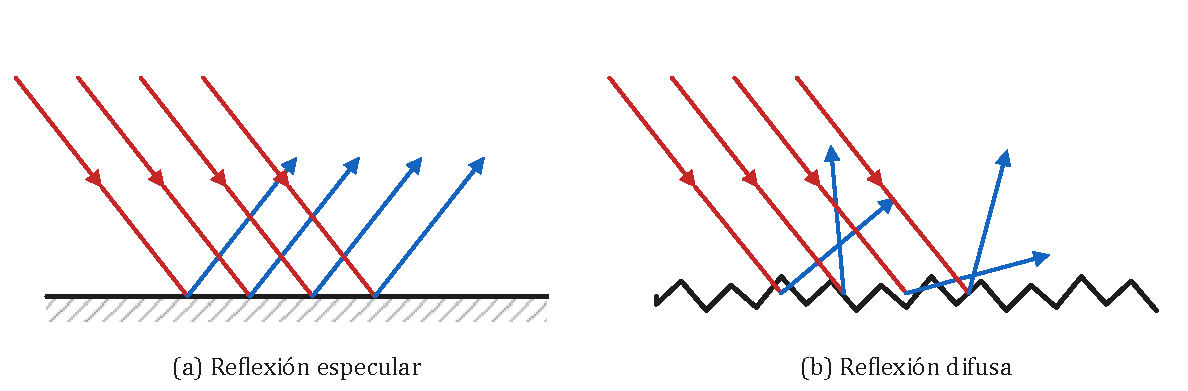
\includegraphics[width=0.85\linewidth]{images/UD3/reflexion_tipos}
    \caption{En una superficie pulida los rayos reflejados siguen paralelos; en una rugosa se dispersan.}
    \label{fig:opt-reflexion}
\end{figure}

Las \textbf{leyes de la reflexión}, que ya vimos para las ondas en la unidad anterior, son:
\begin{enumerate}[label=\numberballmDarkTeal]
    \item El rayo incidente, la normal y el rayo reflejado están en el mismo plano.
    \item El ángulo de incidencia es igual al de reflexión: \(\hat{\imath} = \hat r\).
\end{enumerate}

\subsection{Refracción. Ley de Snell}\label{subsec:opt-snell}

La \rojon{refracción} es el cambio de dirección de la luz al pasar de un medio a otro en el que tiene distinta velocidad.
Por ella un lápiz parece quebrado dentro de un vaso de agua o un pez parece estar más arriba de donde está. Las leyes son:
\begin{enumerate}[label=\numberballmDarkTeal]
    \item El rayo incidente, la normal y el rayo refractado están en el mismo plano.
    \item Se cumple la \rojon{ley de Snell}. Como \(v = c/n\):
    \begin{equation*}
        \dfrac{\sen\hat{\imath}}{\sen\hat r} = \dfrac{v_1}{v_2} = \dfrac{c/n_1}{c/n_2} = \dfrac{n_2}{n_1}
    \end{equation*}
    \begin{centeredequation}
        \boxed{n_1\sen\hat{\imath} = n_2\sen\hat r} \label{eq:opt-snell}
    \end{centeredequation}
\end{enumerate}

Si la luz pasa a un medio \textbf{más} refringente (\(n_2 > n_1\)), \(\sen\hat r < \sen\hat{\imath}\): el rayo se
\textbf{acerca} a la normal. Si pasa a uno \textbf{menos} refringente, se \textbf{aleja} de ella
(figura~\ref{fig:opt-refraccion}).

\begin{figure}[H]
    \centering
    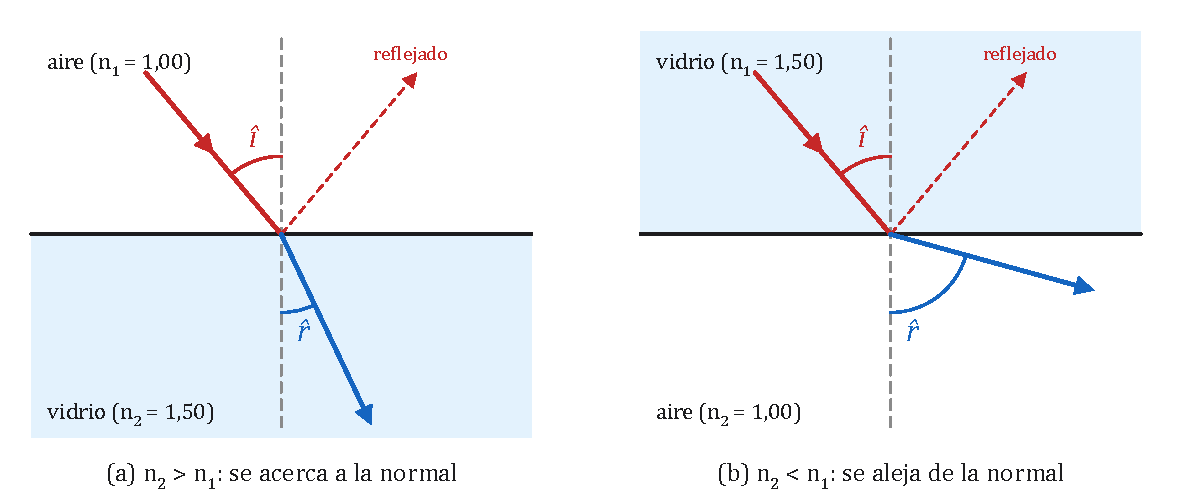
\includegraphics[width=0.92\linewidth]{images/UD3/refraccion_luz}
    \caption{Refracción entre aire y vidrio en los dos sentidos. En la superficie también se refleja parte de la luz.}
    \label{fig:opt-refraccion}
\end{figure}

\begin{exercise}
    Un rayo de luz pasa de un medio de índice \num{1.60} a otro de índice \num{1.40} con un ángulo de incidencia de \ang{35}.
    ¿Cuánto vale el ángulo de refracción? ¿Se acerca o se aleja de la normal?
    \begin{solu}
        \(\sen\hat r = \dfrac{n_1}{n_2}\sen\hat{\imath} = \dfrac{1{,}60}{1{,}40}\sen\ang{35} = 0{,}656 \Rightarrow \textcolor{red}{\hat r = \ang{41.0}}\):
        \textcolor{red}{se aleja de la normal}, \textcolor{blue}{porque pasa a un medio menos refringente.}
    \end{solu}
\end{exercise}

\begin{exercise}
    ¿Qué le ocurre a un rayo que llega perpendicularmente a la superficie de separación de dos medios?
    \begin{solu}
        \textcolor{blue}{Si \(\hat{\imath} = 0\), la ley de Snell da \(\sen\hat r = 0\):} \textcolor{red}{no se desvía},
        aunque \textcolor{red}{sí cambian su velocidad y su longitud de onda.}
    \end{solu}
\end{exercise}

\subsection{Ángulo límite y reflexión total}\label{subsec:opt-limite}

Cuando la luz pasa de un medio a otro \textbf{menos} refringente (\(n_1 > n_2\)), el ángulo de refracción es mayor que el
de incidencia. Si vamos aumentando \(\hat{\imath}\), llega un momento en que el rayo refractado sale rasante a la superficie
(\(\hat r = \ang{90}\)). Ese ángulo de incidencia es el \rojon{ángulo límite} \(\hat{\imath}_L\):
\begin{centeredequation}
    n_1\sen\hat{\imath}_L = n_2\sen\ang{90} \qquad\Rightarrow\qquad \boxed{\sen\hat{\imath}_L = \dfrac{n_2}{n_1}} \label{eq:opt-limite}
\end{centeredequation}
Para ángulos de incidencia mayores que el límite no hay rayo refractado: toda la luz se refleja. Es la \rojon{reflexión
total} (figura~\ref{fig:opt-limite}).

\begin{figure}[H]
    \centering
    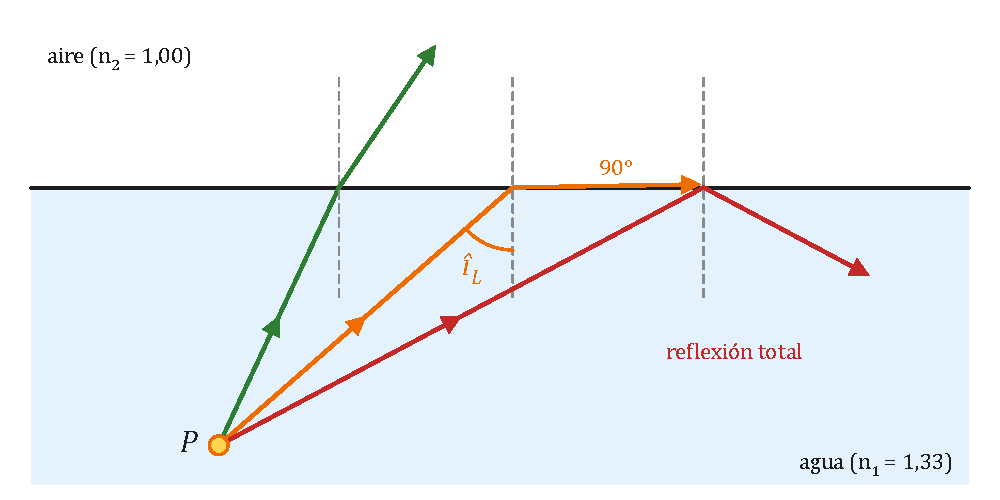
\includegraphics[width=0.62\linewidth]{images/UD3/angulo_limite}
    \caption{Rayos que salen de un punto sumergido. El rayo 2 incide con el ángulo límite y sale rasante; el 3, con un
    ángulo mayor, se refleja totalmente.}
    \label{fig:opt-limite}
\end{figure}

\begin{remark}
    La reflexión total solo es posible cuando la luz va hacia un medio \textbf{menos} refringente. Se aprovecha en la
    \textbf{fibra óptica}: la luz entra en un hilo de vidrio muy fino y avanza rebotando en sus paredes sin salir, aunque
    la fibra se curve. También en los prismas de los prismáticos y en el brillo de los diamantes, cuyo ángulo límite es muy
    pequeño (unos \ang{24}).
\end{remark}

\begin{exercise}
    ¿Cuál es el ángulo de incidencia mínimo para que la luz que va del agua (\(n = 1{,}33\)) al aire se refleje totalmente?
    \begin{solu}
        \(\sen\hat{\imath}_L = \dfrac{1}{1{,}33} = 0{,}752 \Rightarrow \textcolor{red}{\hat{\imath}_L = \ang{48.8}}\).
    \end{solu}
\end{exercise}

\begin{exercise}
    Un diamante (\(n = 2{,}42\)) sumergido en cierto líquido tiene un ángulo límite de \ang{34}. Calcula el índice de
    refracción del líquido y la velocidad de la luz en él.
    \begin{solu}
        \(n_{\text{liq}} = n_{\text{diam}}\sen\hat{\imath}_L = 2{,}42\sen\ang{34} = \textcolor{red}{1{,}35}\);
        \(v = \dfrac{c}{n} = \textcolor{red}{\qty{2.22e8}{\m\per\second}}\).
    \end{solu}
\end{exercise}

\begin{exercise}
    Una fibra óptica de cuarzo tiene un índice de refracción de \num{1.46}. ¿A qué velocidad viaja la luz por ella? ¿Cuál es
    el ángulo límite si la fibra está rodeada de aire?
    \begin{solu}
        \(v = \dfrac{3\cdot 10^8}{1{,}46} = \textcolor{red}{\qty{2.05e8}{\m\per\second}}\);
        \(\sen\hat{\imath}_L = \dfrac{1}{1{,}46} \Rightarrow \textcolor{red}{\hat{\imath}_L = \ang{43.2}}\).
    \end{solu}
\end{exercise}

\subsection{Lámina de caras planas y paralelas}\label{subsec:opt-lamina}

Una lámina transparente de caras paralelas (una ventana, un portaobjetos) refracta la luz dos veces
(figura~\ref{fig:opt-lamina}). Si a los dos lados hay el mismo medio:
\begin{equation*}
    n_1\sen\hat{\imath}_1 = n\sen\hat r_1 \quad\text{(primera cara)}, \qquad n\sen\hat r_1 = n_1\sen\hat{\imath}_2 \quad\text{(segunda cara)}
    \;\Rightarrow\; \hat{\imath}_1 = \hat{\imath}_2
\end{equation*}
\textbf{El rayo emergente es paralelo al incidente}, pero sale desplazado una distancia \(\delta\). Si \(e\) es el espesor de
la lámina, el camino recorrido dentro es \(AB = e/\cos\hat r_1\), y en el triángulo que forman \(AB\) y \(\delta\):
\begin{centeredequation}
    \boxed{\delta = AB\sen(\hat{\imath}_1 - \hat r_1) = e\,\dfrac{\sen(\hat{\imath}_1 - \hat r_1)}{\cos\hat r_1}} \label{eq:opt-lamina}
\end{centeredequation}

\begin{figure}[H]
    \centering
    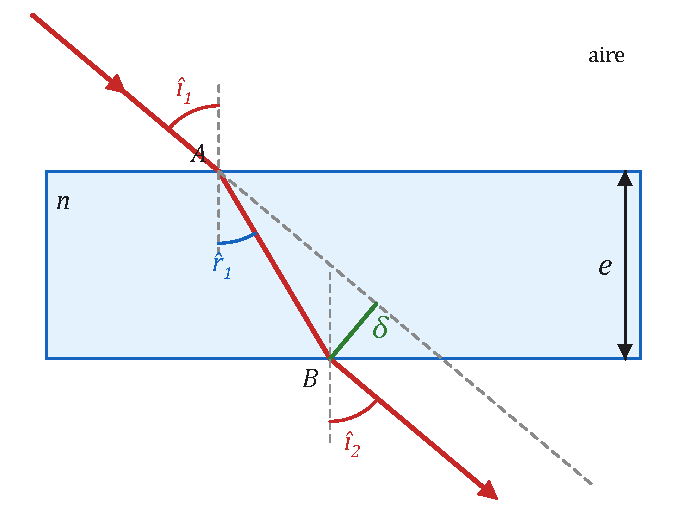
\includegraphics[width=0.48\linewidth]{images/UD3/lamina}
    \caption{Marcha de un rayo a través de una lámina de caras paralelas de espesor \(e\).}
    \label{fig:opt-lamina}
\end{figure}

\begin{exercise}
    Sobre una lámina de vidrio de \qty{2}{\cm} de espesor e índice \num{1.52}, situada en el aire, incide un rayo con un
    ángulo de \ang{40}. Calcula el ángulo de refracción dentro de la lámina, el ángulo de emergencia, el desplazamiento
    lateral y la distancia que recorre el rayo dentro del vidrio.
    \begin{solu}
        \(\sen\hat r_1 = \dfrac{\sen\ang{40}}{1{,}52} = 0{,}423 \Rightarrow \textcolor{red}{\hat r_1 = \ang{25.0}}\);
        \textcolor{red}{emerge con \ang{40}} \textcolor{blue}{(paralelo al incidente).}

        \(AB = \dfrac{2}{\cos\ang{25.0}} = \textcolor{red}{\qty{2.21}{\cm}}\);
        \(\delta = 2{,}21\sen(\ang{40} - \ang{25.0}) = \textcolor{red}{\qty{0.57}{\cm}}\).
    \end{solu}
\end{exercise}

\subsection{El prisma óptico}\label{subsec:opt-prisma}

Un \rojon{prisma óptico} es un medio transparente limitado por dos caras planas que forman un ángulo \(\varphi\), el
\azuln{ángulo del prisma}. Un rayo que entra por una cara se refracta dos veces y sale desviado hacia la base un ángulo
\(\delta\), el \azuln{ángulo de desviación} (figura~\ref{fig:opt-prisma}).

\begin{figure}[H]
    \centering
    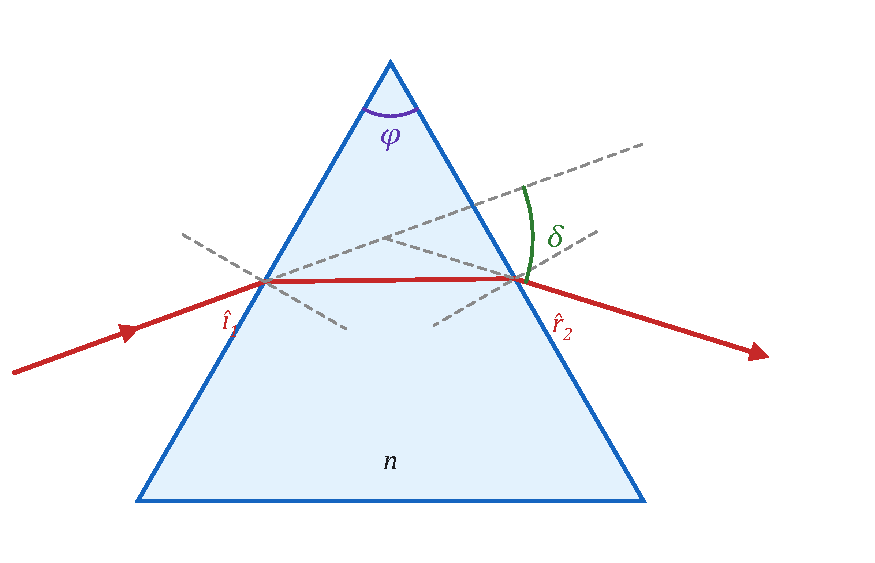
\includegraphics[width=0.55\linewidth]{images/UD3/prisma}
    \caption{Marcha de un rayo en un prisma de ángulo \(\varphi\). La desviación \(\delta\) es el ángulo entre la
    prolongación del rayo incidente y el rayo emergente.}
    \label{fig:opt-prisma}
\end{figure}

Si el prisma está en el aire, en cada cara se cumple la ley de Snell:
\begin{equation*}
    \sen\hat{\imath}_1 = n\sen\hat r_1 \qquad\qquad n\sen\hat{\imath}_2 = \sen\hat r_2
\end{equation*}
Las dos normales forman entre sí el mismo ángulo \(\varphi\) que las caras, y la geometría del triángulo que forman con el
rayo interior da:
\begin{centeredequation}
    \boxed{\varphi = \hat r_1 + \hat{\imath}_2} \qquad\qquad \boxed{\delta = \hat{\imath}_1 + \hat r_2 - \varphi} \label{eq:opt-prisma}
\end{centeredequation}

\paragraph{Desviación mínima.} La desviación depende del ángulo de incidencia y es \textbf{mínima} cuando el rayo atraviesa
el prisma simétricamente, paralelo a la base: entonces \(\hat{\imath}_1 = \hat r_2\) y \(\hat r_1 = \hat{\imath}_2 = \varphi/2\).
Con \(\delta_m = 2\hat{\imath}_1 - \varphi\):
\begin{centeredequation}
    \hat{\imath}_1 = \dfrac{\delta_m + \varphi}{2} \qquad\Rightarrow\qquad \boxed{n = \dfrac{\sen\dfrac{\delta_m + \varphi}{2}}{\sen\dfrac{\varphi}{2}}} \label{eq:opt-desviacion-minima}
\end{centeredequation}
Como \(\varphi\) y \(\delta_m\) se miden con facilidad, esta fórmula permite determinar en el laboratorio el índice de
refracción de un material tallado en forma de prisma.

\begin{exercise}
    Calcula la desviación mínima que produce un prisma equilátero (\(\varphi = \ang{60}\)) de vidrio de índice \num{1.5}.
    \begin{solu}
        \textcolor{blue}{En la desviación mínima \(\hat r_1 = \ang{30}\):} \(\sen\hat{\imath}_1 = 1{,}5\sen\ang{30} = 0{,}75 \Rightarrow \hat{\imath}_1 = \ang{48.6}\).
        \[ \delta_m = 2\hat{\imath}_1 - \varphi = 2\cdot\ang{48.6} - \ang{60} = \textcolor{red}{\ang{37.2}} \]
    \end{solu}
\end{exercise}

\subsection{Dispersión de la luz}\label{subsec:opt-dispersion}

La luz blanca es una mezcla de luces de distintas longitudes de onda (colores). En el vacío todas viajan a la misma
velocidad, pero en un medio material el índice de refracción depende ligeramente de la longitud de onda: es mayor para la
luz violeta (\(\lambda\) corta) que para la roja (\(\lambda\) larga). Por eso, al atravesar un prisma, cada color se desvía un
ángulo distinto y la luz blanca se separa en un abanico de colores, el \azuln{espectro visible}. Este fenómeno es la
\rojon{dispersión} de la luz (figura~\ref{fig:opt-dispersion}).

\begin{figure}[H]
    \centering
    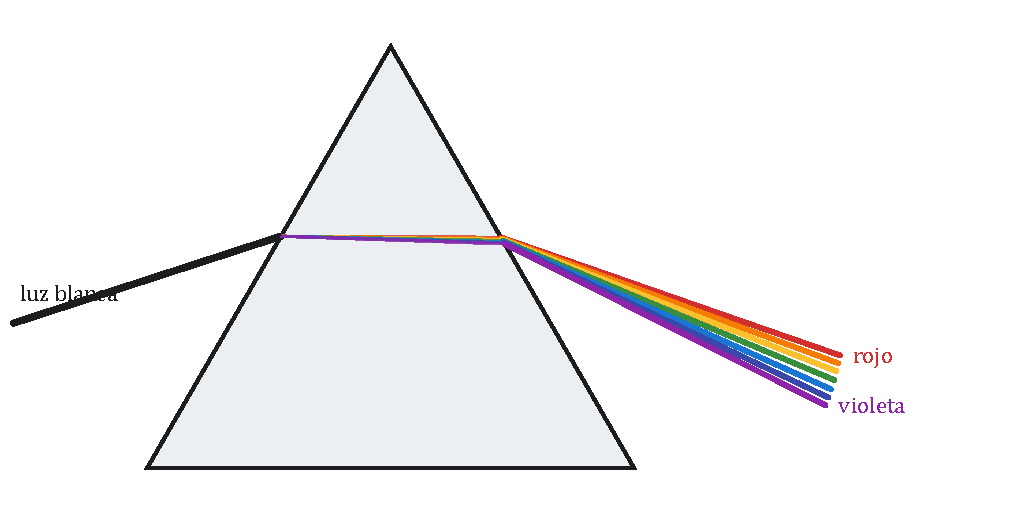
\includegraphics[width=0.66\linewidth]{images/UD3/dispersion}
    \caption{Dispersión de la luz blanca en un prisma: el violeta, con mayor índice de refracción, es el que más se desvía
    (la separación entre colores está exagerada).}
    \label{fig:opt-dispersion}
\end{figure}

El \textbf{arco iris} es un ejemplo natural: la luz del Sol se refracta al entrar en cada gota de lluvia, se refleja en su
parte posterior y vuelve a refractarse al salir, separándose en colores. Lo vemos cuando tenemos el Sol a la espalda y
llueve delante de nosotros, con el rojo en la parte exterior del arco y el violeta en la interior.

\section{Conceptos básicos de óptica geométrica}\label{sec:opt-conceptos}

La óptica geométrica estudia la formación de imágenes usando solo el concepto de rayo, sin tener en cuenta la naturaleza
ondulatoria de la luz. Se basa en cuatro hechos:
\begin{itemize}
    \item En un medio homogéneo e isótropo la luz se propaga en línea recta.
    \item Los rayos son independientes: si se cruzan, cada uno sigue su camino.
    \item Se cumplen las leyes de la reflexión y de la refracción.
    \item Los caminos son reversibles: si un rayo va de \(P\) a \(P'\), otro que salga de \(P'\) en sentido contrario
    llega a \(P\) por el mismo camino.
\end{itemize}

\paragraph{Definiciones.}
\begin{itemize}
    \item \textbf{Dioptrio}: superficie que separa dos medios transparentes de distinto índice de refracción. Puede ser
    plano o esférico.
    \item \textbf{Sistema óptico}: conjunto de dioptrios (y espejos). Su \azuln{eje óptico} o eje principal es la recta
    común que pasa por los centros de todas las superficies.
    \item En un dioptrio esférico, el \azuln{centro de curvatura} \(C\) es el centro de la esfera, \(R\) es su radio y el
    \azuln{vértice} \(O\) es el punto donde la superficie corta al eje.
    \item \textbf{Imagen real}: los rayos que salen de un punto objeto \(A\) se cortan, después de atravesar el sistema, en
    un punto \(A'\). Se puede recoger en una pantalla.
    \item \textbf{Imagen virtual}: los rayos salen divergentes y son sus \emph{prolongaciones} hacia atrás las que se cortan
    en \(A'\). No se puede recoger en una pantalla, pero el ojo la ve (como la imagen de un espejo plano).
\end{itemize}

\subsection{Convenio de signos}\label{subsec:opt-signos}

Usaremos el convenio de las normas \textbf{DIN}:
\begin{itemize}
    \item La luz llega siempre desde la \textbf{izquierda}.
    \item Las distancias horizontales se miden desde el vértice \(O\) (o el centro óptico): son \textbf{positivas hacia
    la derecha} y negativas hacia la izquierda. Por eso un objeto real situado delante del sistema tiene \(s < 0\).
    \item Las distancias verticales se miden desde el eje: positivas hacia arriba y negativas hacia abajo.
    \item Las magnitudes de la imagen se escriben con prima: \(s'\), \(y'\), \(f'\)\ldots
    \item El radio \(R\) es positivo si el centro de curvatura está a la derecha del vértice (superficie convexa vista
    desde la luz que llega) y negativo si está a la izquierda (cóncava).
\end{itemize}

\begin{remark}
    Los resultados de esta unidad valen para \textbf{rayos paraxiales}, los que forman ángulos pequeños con el eje (menos
    de unos \ang{10}). Para ellos \(\sen\alpha \approx \tg\alpha \approx \alpha\), y todos los rayos que salen de un punto
    se cortan en un único punto imagen.
\end{remark}

\section{El dioptrio esférico}\label{sec:opt-dioptrio}

Consideremos un dioptrio esférico de radio \(R\) que separa un medio de índice \(n\) (a la izquierda) de otro de índice
\(n'\). Un rayo sale de un punto \(A\) del eje, a una distancia \(s\) del vértice, se refracta en un punto \(P\) situado a
una altura \(h\) y corta al eje en \(A'\), a una distancia \(s'\) (figura~\ref{fig:opt-dioptrio}).

\begin{figure}[H]
    \centering
    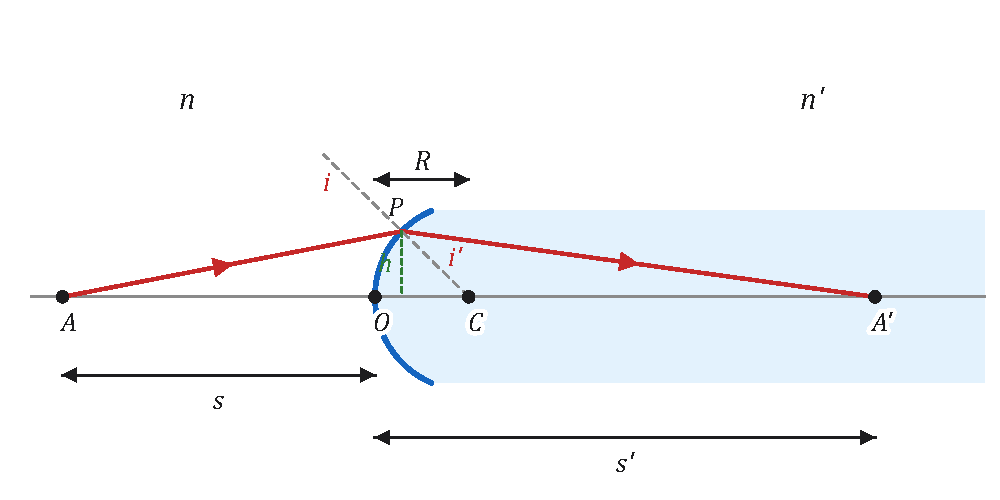
\includegraphics[width=0.66\linewidth]{images/UD3/dioptrio}
    \caption{Refracción en un dioptrio esférico convexo. La normal en \(P\) es la recta que pasa por el centro \(C\).}
    \label{fig:opt-dioptrio}
\end{figure}

Con rayos paraxiales, la ley de Snell queda \(n\,i = n'\,i'\). Los ángulos \(i\) e \(i'\) se pueden expresar con los
ángulos que forman con el eje el rayo incidente, el refractado y la normal, que para ángulos pequeños valen
aproximadamente \(h/s\), \(h/s'\) y \(h/R\). Sustituyendo y dividiendo por \(h\) se obtiene la \rojon{ecuación fundamental
del dioptrio esférico}:
\begin{centeredequation}
    \boxed{\dfrac{n'}{s'} - \dfrac{n}{s} = \dfrac{n' - n}{R}} \label{eq:opt-dioptrio}
\end{centeredequation}
No depende de \(h\): todos los rayos paraxiales que salen de \(A\) pasan por el mismo punto \(A'\).

\paragraph{Focos y distancias focales.}
\begin{itemize}
    \item El \azuln{foco imagen} \(F'\) es el punto donde convergen los rayos que llegan paralelos al eje (objeto en el
    infinito, \(s = -\infty\)). Su distancia al vértice es la \azuln{distancia focal imagen} \(f'\).
    \item El \azuln{foco objeto} \(F\) es el punto del eje del que tienen que salir los rayos para que, tras refractarse,
    salgan paralelos al eje (\(s' = \infty\)). Su distancia al vértice es la \azuln{distancia focal objeto} \(f\).
\end{itemize}
\begin{centeredequation}
    \dfrac{n'}{f'} - \dfrac{n}{-\infty} = \dfrac{n' - n}{R} \Rightarrow f' = R\,\dfrac{n'}{n' - n} \qquad\qquad
    \dfrac{n'}{\infty} - \dfrac{n}{f} = \dfrac{n' - n}{R} \Rightarrow f = -R\,\dfrac{n}{n' - n} \label{eq:opt-focales-dioptrio}
\end{centeredequation}
Se cumplen además \(\dfrac{f}{f'} = -\dfrac{n}{n'}\) y \(f + f' = R\). Dividiendo la ecuación fundamental entre \((n'-n)/R\)
se llega a la \azuln{ecuación de Gauss}: \(\dfrac{f'}{s'} + \dfrac{f}{s} = 1\).

\begin{figure}[H]
    \centering
    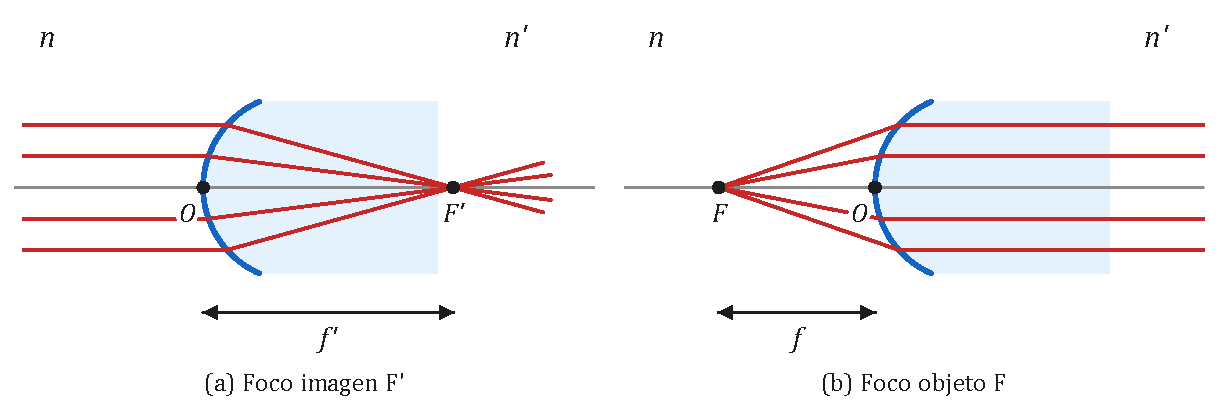
\includegraphics[width=0.9\linewidth]{images/UD3/dioptrio_focos}
    \caption{Focos de un dioptrio esférico convexo con \(n < n'\).}
    \label{fig:opt-dioptrio-focos}
\end{figure}

\paragraph{Construcción de imágenes.} Para hallar la imagen de un objeto \(AB\) perpendicular al eje se trazan desde \(B\)
dos de estos rayos y se busca su corte:
\begin{itemize}
    \item el rayo paralelo al eje, que se refracta pasando por \(F'\);
    \item el rayo que pasa por \(F\), que se refracta saliendo paralelo al eje;
    \item el rayo que pasa por \(C\), que no se desvía (llega perpendicular a la superficie).
\end{itemize}

\paragraph{Aumento lateral.} Es el cociente entre el tamaño de la imagen y el del objeto. Aplicando la ley de Snell al rayo
que llega al vértice:
\begin{centeredequation}
    \boxed{\beta = \dfrac{y'}{y} = \dfrac{n\,s'}{n'\,s}} \label{eq:opt-aumento-dioptrio}
\end{centeredequation}
Si \(\beta > 0\) la imagen es \textbf{derecha}; si \(\beta < 0\), \textbf{invertida}. Si \(|\beta| > 1\), es mayor que el objeto.

\begin{exercise}
    Un dioptrio esférico cóncavo de \qty{20}{\cm} de radio separa el aire (\(n = 1\)) de un vidrio de índice \num{1.5}. A
    \qty{40}{\cm} delante del vértice hay un objeto de \qty{3}{\cm} de altura. Calcula las distancias focales y la posición
    y el tamaño de la imagen.
    \begin{solu}
        \textcolor{blue}{Cóncavo: \(R = \qty{-20}{\cm}\); \(s = \qty{-40}{\cm}\).}

        \(f' = R\,\dfrac{n'}{n' - n} = -20\cdot\dfrac{1{,}5}{0{,}5} = \textcolor{red}{\qty{-60}{\cm}}\);
        \(f = -R\,\dfrac{n}{n' - n} = \textcolor{red}{\qty{40}{\cm}}\).

        \(\dfrac{1{,}5}{s'} = \dfrac{0{,}5}{-20} + \dfrac{1}{-40} = -0{,}05 \Rightarrow \textcolor{red}{s' = \qty{-30}{\cm}}\)
        \textcolor{blue}{(a la izquierda del vértice: imagen virtual).}

        \(\beta = \dfrac{1\cdot(-30)}{1{,}5\cdot(-40)} = 0{,}5 \Rightarrow \textcolor{red}{y' = \qty{1.5}{\cm}}\), \textcolor{red}{derecha y menor}.
    \end{solu}
\end{exercise}

\begin{exercise}
    Un dioptrio esférico convexo de \qty{30}{\cm} de radio separa dos medios de índices \num{1.2} y \num{1.8}. Calcula la
    posición y el tamaño de la imagen de un objeto de \qty{2}{\cm} situado \qty{90}{\cm} a la izquierda del vértice.
    \begin{solu}
        \(\dfrac{1{,}8}{s'} = \dfrac{1{,}8 - 1{,}2}{30} + \dfrac{1{,}2}{-90} = 0{,}02 - 0{,}0133 = 0{,}00667 \Rightarrow \textcolor{red}{s' = \qty{270}{\cm}}\)
        \textcolor{blue}{(imagen real).}

        \(\beta = \dfrac{1{,}2\cdot 270}{1{,}8\cdot(-90)} = -2 \Rightarrow \textcolor{red}{y' = \qty{-4}{\cm}}\): \textcolor{red}{invertida y el doble de grande}.
    \end{solu}
\end{exercise}

\subsection{El dioptrio plano}\label{subsec:opt-dioptrio-plano}

Un dioptrio plano es un dioptrio esférico de radio infinito. Con \(R = \infty\) la ecuación fundamental queda:
\begin{centeredequation}
    \dfrac{n'}{s'} = \dfrac{n}{s} \qquad\Rightarrow\qquad \boxed{\dfrac{s'}{s} = \dfrac{n'}{n}} \label{eq:opt-dioptrio-plano}
\end{centeredequation}
y el aumento es \(\beta = \dfrac{n s'}{n' s} = 1\): la imagen tiene el mismo tamaño que el objeto. Explica la
\textbf{profundidad aparente}: un objeto sumergido se ve más cerca de la superficie de lo que está, porque \(n' = 1 < n\) y
\(|s'| < |s|\) (figura~\ref{fig:opt-profundidad}).

\begin{figure}[H]
    \centering
    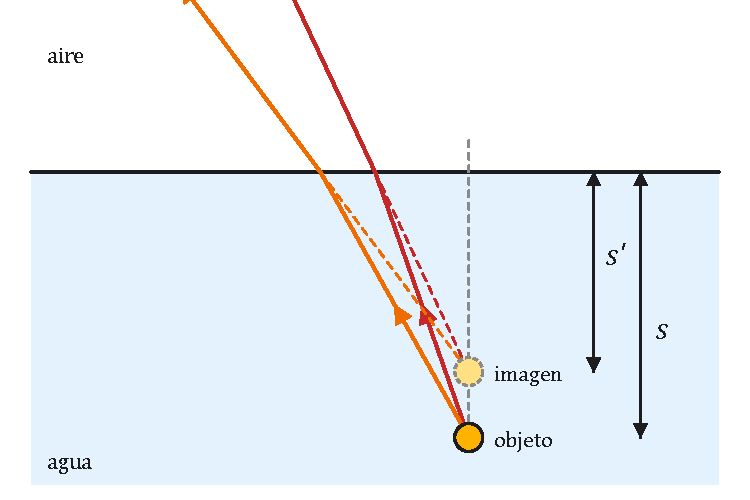
\includegraphics[width=0.5\linewidth]{images/UD3/profundidad}
    \caption{Los rayos que salen del objeto se alejan de la normal al salir al aire. Sus prolongaciones se cortan más arriba:
    el objeto parece estar a una profundidad \(s'\) menor que la real.}
    \label{fig:opt-profundidad}
\end{figure}

\begin{exercise}
    Un buceador mira hacia arriba desde el fondo de un embalse y ve un helicóptero que vuela a \qty{250}{\m} sobre el agua
    (\(n_{\text{agua}} = 1{,}33\)). ¿A qué altura le parece que está?
    \begin{solu}
        \textcolor{blue}{La luz va del aire (\(n = 1\)) al agua (\(n' = 1{,}33\)):}
        \(s' = s\,\dfrac{n'}{n} = 250\cdot 1{,}33 = \textcolor{red}{\qty{332.5}{\m}}\): \textcolor{blue}{lo ve más alto de lo que está.}
    \end{solu}
\end{exercise}

\begin{exercise}
    ¿A qué profundidad parece estar una moneda en el fondo de una piscina de \qty{2.2}{\m} llena de agua (\(n = 1{,}33\))?
    \begin{solu}
        \textcolor{blue}{Ahora la luz va del agua (\(n = 1{,}33\)) al aire (\(n' = 1\)):}
        \(s' = s\,\dfrac{n'}{n} = \dfrac{2{,}2}{1{,}33} = \textcolor{red}{\qty{1.65}{\m}}\).
    \end{solu}
\end{exercise}

\section{Espejos}\label{sec:opt-espejos}

Un espejo es una superficie que refleja casi toda la luz que le llega (normalmente, vidrio con una capa de plata o de
aluminio por detrás). La reflexión puede tratarse como una refracción especial: la luz sigue en el mismo medio, pero
cambia de sentido. Basta tomar \(n' = -n\) en las fórmulas del dioptrio.

\subsection{Espejo plano}\label{subsec:opt-espejo-plano}

Con \(n' = -n\) en la ecuación del dioptrio plano:
\begin{equation*}
    \dfrac{s'}{s} = \dfrac{-n}{n} = -1 \qquad\Rightarrow\qquad \boxed{s' = -s} \qquad\qquad \beta = 1
\end{equation*}
Un espejo plano da una imagen \textbf{virtual} (está detrás del espejo), \textbf{derecha}, del \textbf{mismo tamaño} y a la
\textbf{misma distancia} que el objeto (figura~\ref{fig:opt-espejo-plano}). Además, la imagen está invertida de izquierda a
derecha: la imagen de una mano derecha es una mano izquierda.

\begin{figure}[H]
    \centering
    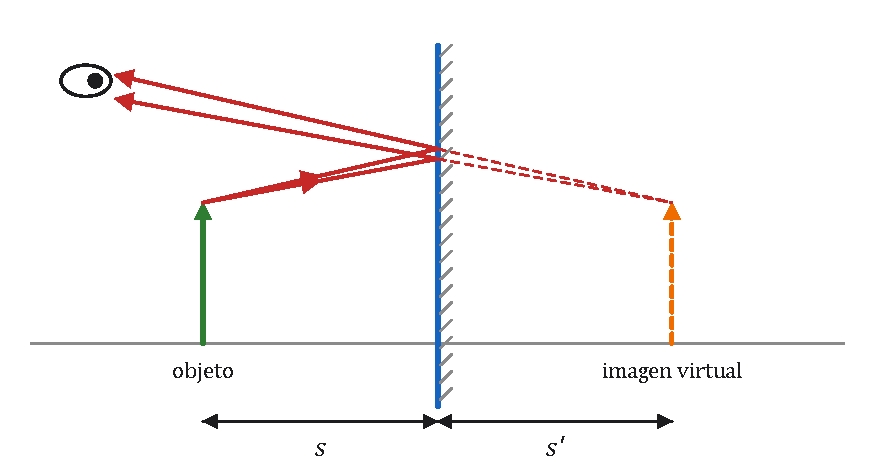
\includegraphics[width=0.56\linewidth]{images/UD3/espejo_plano}
    \caption{Los rayos reflejados que llegan al ojo parecen salir de un punto situado detrás del espejo.}
    \label{fig:opt-espejo-plano}
\end{figure}

\begin{exercise}
    ¿Qué altura mínima debe tener un espejo plano vertical para que una persona de \qty{1.70}{\m} se vea entera? ¿Depende
    de la distancia a la que se ponga?
    \begin{solu}
        \textcolor{blue}{Los rayos que van de la cabeza y de los pies a los ojos se reflejan en el espejo a mitad de camino
        entre cada punto y los ojos (la imagen está igual de lejos que la persona). Entre esos dos puntos de reflexión hay la
        mitad de la altura de la persona.}
        \textcolor{red}{El espejo debe medir \qty{0.85}{\m}} (la mitad de la altura), con su borde superior a media distancia
        entre los ojos y la coronilla. \textcolor{red}{No depende de la distancia al espejo.}
    \end{solu}
\end{exercise}

\subsection{Espejos esféricos}\label{subsec:opt-espejos-esfericos}

Un espejo esférico es un casquete de esfera que refleja la luz. Es \azuln{cóncavo} si la superficie reflectante es la
interior (su centro de curvatura está delante, a la izquierda: \(R < 0\)) y \azuln{convexo} si es la exterior (\(R > 0\)).

\paragraph{Foco y distancia focal.} Con \(n' = -n\) en las distancias focales del dioptrio:
\(f' = R\,\dfrac{-n}{-2n} = \dfrac{R}{2}\) y \(f = -R\,\dfrac{n}{-2n} = \dfrac{R}{2}\). En un espejo los dos focos coinciden en
un único punto \(F\), a mitad de camino entre el vértice y el centro de curvatura:
\begin{centeredequation}
    \boxed{f = f' = \dfrac{R}{2}} \label{eq:opt-focal-espejo}
\end{centeredequation}
En un espejo cóncavo los rayos que llegan paralelos al eje se reflejan pasando por \(F\) (\(f < 0\)); en uno convexo, son
sus prolongaciones las que pasan por \(F\), detrás del espejo (\(f > 0\), figura~\ref{fig:opt-espejos-foco}).

\begin{figure}[H]
    \centering
    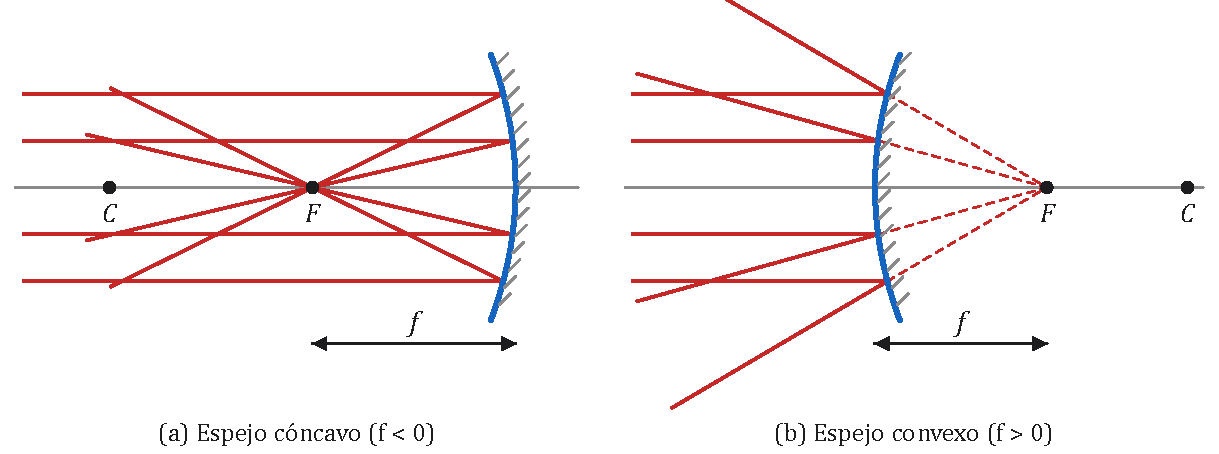
\includegraphics[width=0.9\linewidth]{images/UD3/espejos_foco}
    \caption{Foco de un espejo cóncavo (real) y de uno convexo (virtual).}
    \label{fig:opt-espejos-foco}
\end{figure}

\paragraph{Ecuación de los espejos y aumento.} Con \(n' = -n\) en la ecuación del dioptrio y dividiendo por \(-n\):
\begin{equation*}
    \dfrac{-n}{s'} - \dfrac{n}{s} = \dfrac{-2n}{R} \qquad\Rightarrow\qquad \dfrac{1}{s'} + \dfrac{1}{s} = \dfrac{2}{R}
\end{equation*}
\begin{centeredequation}
    \boxed{\dfrac{1}{s'} + \dfrac{1}{s} = \dfrac{1}{f}} \qquad\qquad \boxed{\beta = \dfrac{y'}{y} = -\dfrac{s'}{s}} \label{eq:opt-espejos}
\end{centeredequation}
Con el convenio de signos: si \(s' < 0\) la imagen está delante del espejo y es \textbf{real}; si \(s' > 0\), está detrás y
es \textbf{virtual}.

\paragraph{Construcción de imágenes.} Se usan dos de estos tres rayos que salen del extremo del objeto:
\begin{itemize}
    \item el que llega \textbf{paralelo al eje} se refleja pasando por \(F\) (en el convexo, su prolongación pasa por \(F\));
    \item el que pasa (o se dirige) \textbf{por el foco} se refleja paralelo al eje;
    \item el que pasa (o se dirige) \textbf{por el centro de curvatura} se refleja sobre sí mismo.
\end{itemize}

\begin{figure}[H]
    \centering
    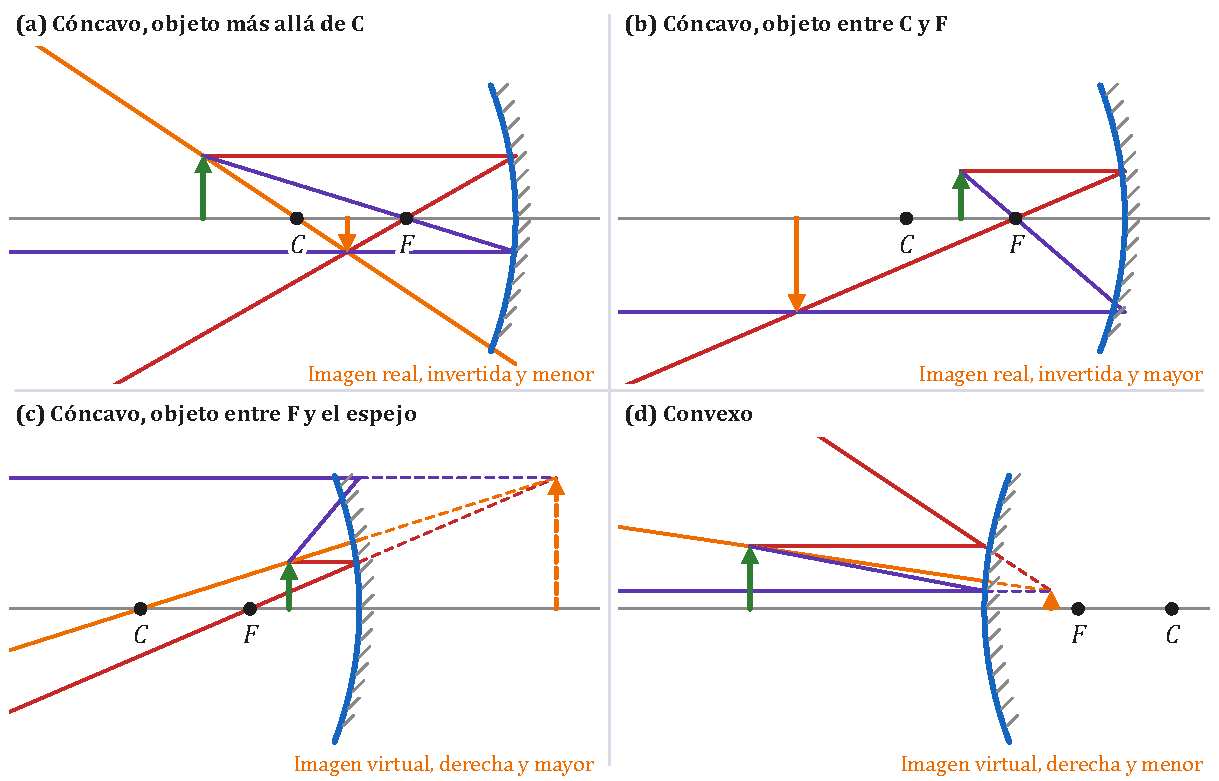
\includegraphics[width=\linewidth]{images/UD3/espejos_imagenes}
    \caption{Imágenes en espejos esféricos (objeto en verde, imagen en naranja; la imagen virtual, en discontinuo). Un espejo
    convexo siempre da una imagen virtual, derecha y menor, con un campo de visión amplio: por eso se usa en los
    retrovisores y en los cruces sin visibilidad.}
    \label{fig:opt-espejos-imagenes}
\end{figure}

\begin{table}[H]
    \centering
    \caption{Imagen que da un espejo cóncavo según la posición del objeto}
    \vspace{-5pt}
    \begin{tabular}{@{}lll@{}}
        \toprule
        \textbf{Posición del objeto} & \textbf{Posición de la imagen} & \textbf{Características} \\
        \midrule
        Más allá de \(C\) & Entre \(C\) y \(F\) & Real, invertida y menor \\[3pt]
        En \(C\) & En \(C\) & Real, invertida e igual \\[3pt]
        Entre \(C\) y \(F\) & Más allá de \(C\) & Real, invertida y mayor \\[3pt]
        En \(F\) & En el infinito & No se forma imagen \\[3pt]
        Entre \(F\) y el espejo & Detrás del espejo & Virtual, derecha y mayor \\
        \bottomrule
    \end{tabular}
    \label{tab:opt-espejo-concavo}
\end{table}

\begin{exercise}
    Construye la imagen de un objeto colocado en el centro de curvatura de un espejo cóncavo.
    \begin{solu}
        \textcolor{blue}{El rayo paralelo al eje se refleja por \(F\); el que pasa por \(F\) vuelve paralelo. Se cortan
        justo debajo de \(C\), a la misma distancia del eje que el extremo del objeto. Con la ecuación: \(s = R = 2f\),}
        \(\dfrac{1}{s'} = \dfrac{1}{f} - \dfrac{1}{2f} = \dfrac{1}{2f} \Rightarrow s' = 2f = R\), \(\beta = -1\).
        \textcolor{red}{La imagen está en \(C\) y es real, invertida y del mismo tamaño.}
    \end{solu}
\end{exercise}

\begin{exercise}
    Un objeto de \qty{1}{\cm} está a \qty{15}{\cm} a la izquierda de un espejo convexo de \qty{30}{\cm} de radio. Calcula
    la posición, el tamaño y las características de la imagen.
    \begin{solu}
        \textcolor{blue}{\(R = \qty{30}{\cm} \Rightarrow f = \qty{15}{\cm}\); \(s = \qty{-15}{\cm}\).}
        \(\dfrac{1}{s'} = \dfrac{1}{15} - \dfrac{1}{-15} = \dfrac{2}{15} \Rightarrow \textcolor{red}{s' = \qty{7.5}{\cm}}\);
        \(\beta = -\dfrac{7{,}5}{-15} = 0{,}5 \Rightarrow \textcolor{red}{y' = \qty{0.5}{\cm}}\).
        \textcolor{red}{Virtual (detrás del espejo), derecha y de la mitad de tamaño.}
    \end{solu}
\end{exercise}

\begin{exercise}
    Un objeto de \qty{2}{\cm} de altura está a \qty{75}{\cm} de un espejo cóncavo de \qty{50}{\cm} de radio. Calcula la
    distancia focal y la posición y el tamaño de la imagen.
    \begin{solu}
        \textcolor{blue}{\(R = \qty{-50}{\cm}\):} \(f = \dfrac{R}{2} = \textcolor{red}{\qty{-25}{\cm}}\).
        \(\dfrac{1}{s'} = \dfrac{1}{-25} - \dfrac{1}{-75} = -\dfrac{2}{75} \Rightarrow \textcolor{red}{s' = \qty{-37.5}{\cm}}\).

        \(\beta = -\dfrac{-37{,}5}{-75} = -0{,}5 \Rightarrow \textcolor{red}{y' = \qty{-1}{\cm}}\): \textcolor{red}{real, invertida y menor}.
    \end{solu}
\end{exercise}

\begin{exercise}
    Resuelve la actividad anterior si el espejo es convexo.
    \begin{solu}
        \textcolor{blue}{\(R = \qty{50}{\cm}\):} \(f = \textcolor{red}{\qty{25}{\cm}}\).
        \(\dfrac{1}{s'} = \dfrac{1}{25} + \dfrac{1}{75} = \dfrac{4}{75} \Rightarrow \textcolor{red}{s' = \qty{18.75}{\cm}}\);
        \(\beta = 0{,}25 \Rightarrow \textcolor{red}{y' = \qty{0.5}{\cm}}\): \textcolor{red}{virtual, derecha y menor}.
    \end{solu}
\end{exercise}

\section{Lentes delgadas}\label{sec:opt-lentes}

Una \rojon{lente} es un medio transparente limitado por dos superficies, al menos una de ellas esférica: es un sistema de
dos dioptrios. Si su espesor es pequeño comparado con los radios de curvatura, es una \azuln{lente delgada}, y se puede
considerar que los dos vértices coinciden en un único punto, el \azuln{centro óptico} \(O\).
\begin{itemize}
    \item Las \textbf{lentes convergentes} son más gruesas en el centro que en los bordes: biconvexas, planoconvexas y
    meniscos convergentes. Los rayos paralelos al eje convergen en el foco imagen.
    \item Las \textbf{lentes divergentes} son más gruesas en los bordes: bicóncavas, planocóncavas y meniscos divergentes.
    Los rayos paralelos salen separándose, como si vinieran del foco imagen.
\end{itemize}

\begin{figure}[H]
    \centering
    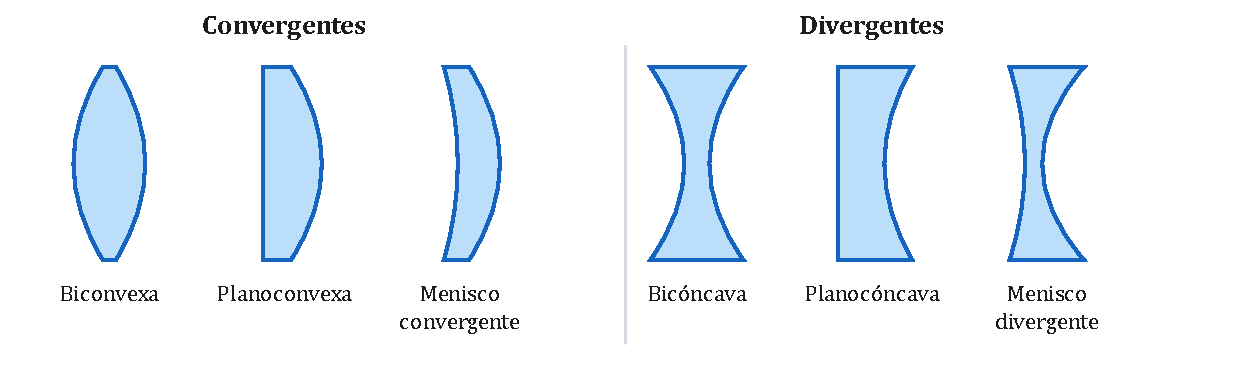
\includegraphics[width=0.9\linewidth]{images/UD3/lentes_tipos}
    \caption{Tipos de lentes. En los esquemas, una lente delgada se representa con un segmento con puntas de flecha
    (convergente) o con las puntas hacia dentro (divergente).}
    \label{fig:opt-lentes-tipos}
\end{figure}

\paragraph{Ecuación del constructor de lentes.} Aplicando la ecuación del dioptrio a las dos caras de una lente de índice
\(n\) en el aire (la imagen de la primera cara hace de objeto para la segunda) y sumando se obtiene:
\begin{centeredequation}
    \dfrac{1}{s'} - \dfrac{1}{s} = (n - 1)\left(\dfrac{1}{R_1} - \dfrac{1}{R_2}\right) \label{eq:opt-constructor}
\end{centeredequation}
Si el objeto está en el infinito, la imagen se forma en el foco imagen, \(s' = f'\):
\begin{centeredequation}
    \dfrac{1}{f'} = (n - 1)\left(\dfrac{1}{R_1} - \dfrac{1}{R_2}\right) \label{eq:opt-focal-lente}
\end{centeredequation}

\paragraph{Ecuación de las lentes delgadas y aumento.} Comparando las dos ecuaciones anteriores:
\begin{centeredequation}
    \boxed{\dfrac{1}{s'} - \dfrac{1}{s} = \dfrac{1}{f'}} \qquad\qquad \boxed{\beta = \dfrac{y'}{y} = \dfrac{s'}{s}} \label{eq:opt-lentes}
\end{centeredequation}
En una lente los dos focos están a ambos lados, a la misma distancia: \(f = -f'\). En una lente convergente \(f' > 0\) (el
foco imagen está a la derecha) y en una divergente \(f' < 0\) (figura~\ref{fig:opt-lentes-focos}). En las lentes, a
diferencia de los espejos, la imagen es \textbf{real} si \(s' > 0\) (se forma detrás de la lente) y \textbf{virtual} si
\(s' < 0\).

\begin{figure}[H]
    \centering
    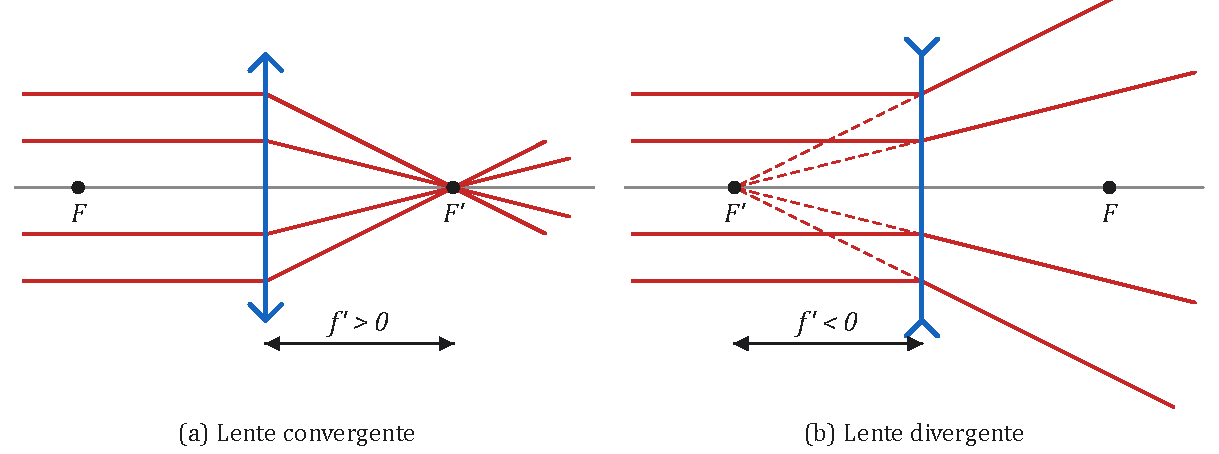
\includegraphics[width=0.9\linewidth]{images/UD3/lentes_focos}
    \caption{Foco imagen \(F'\) de una lente convergente (real) y de una divergente (virtual).}
    \label{fig:opt-lentes-focos}
\end{figure}

\paragraph{Potencia de una lente.} Es la inversa de la distancia focal imagen. Si \(f'\) se mide en metros, la potencia se
mide en \azuln{dioptrías} (\unit{D}, \(\qty{1}{D} = \qty{1}{\per\m}\)):
\begin{centeredequation}
    \boxed{P = \dfrac{1}{f'}} \label{eq:opt-potencia}
\end{centeredequation}
Las lentes convergentes tienen potencia positiva y las divergentes, negativa. Si se ponen varias lentes delgadas juntas, la
potencia del conjunto es la suma: \(P = P_1 + P_2 + \cdots\)

\paragraph{Construcción de imágenes.} Se usan dos de estos tres rayos:
\begin{itemize}
    \item el que llega \textbf{paralelo al eje} sale pasando por \(F'\) (en la divergente, su prolongación pasa por \(F'\));
    \item el que pasa (o se dirige) \textbf{por \(F\)} sale paralelo al eje;
    \item el que pasa por el \textbf{centro óptico} no se desvía.
\end{itemize}

\begin{figure}[H]
    \centering
    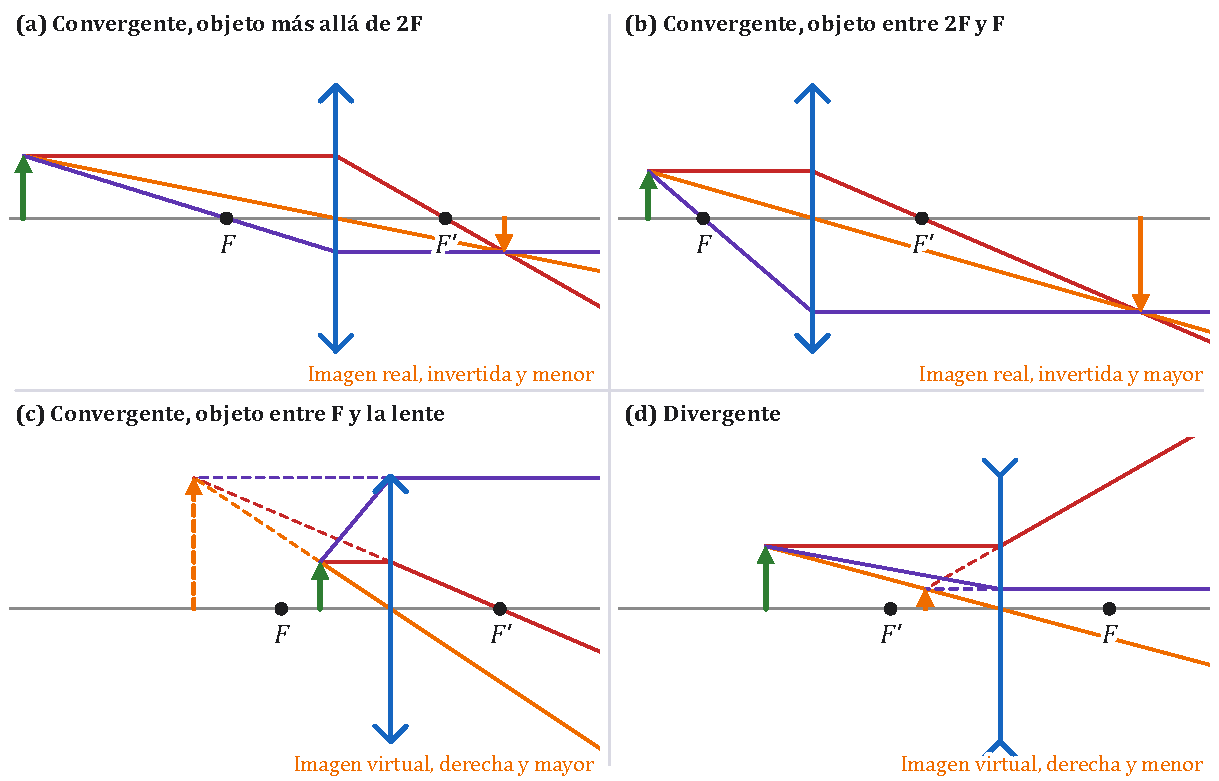
\includegraphics[width=\linewidth]{images/UD3/lentes_imagenes}
    \caption{Imágenes en lentes delgadas. Una lente divergente da siempre una imagen virtual, derecha y menor.}
    \label{fig:opt-lentes-imagenes}
\end{figure}

\begin{exercise}
    Una lente biconvexa de vidrio (\(n = 1{,}5\)) tiene dos caras de \qty{20}{\cm} de radio. Calcula su distancia focal y su
    potencia.
    \begin{solu}
        \textcolor{blue}{Primera cara convexa, \(R_1 = \qty{20}{\cm}\); segunda cóncava vista desde la luz, \(R_2 = \qty{-20}{\cm}\).}
        \[ \dfrac{1}{f'} = 0{,}5\left(\dfrac{1}{20} + \dfrac{1}{20}\right) = 0{,}05\ \unit{\per\cm} \;\Rightarrow\; \textcolor{red}{f' = \qty{20}{\cm}} \]
        \(P = \dfrac{1}{0{,}20} = \textcolor{red}{\qty{5}{D}}\).
    \end{solu}
\end{exercise}

\begin{exercise}
    Un objeto de \qty{3}{\cm} de altura está a \qty{25}{\cm} de una lente convergente de \qty{15}{\cm} de distancia focal.
    Calcula la posición y el tamaño de la imagen.
    \begin{solu}
        \(\dfrac{1}{s'} = \dfrac{1}{15} + \dfrac{1}{-25} = \dfrac{2}{75} \Rightarrow \textcolor{red}{s' = \qty{37.5}{\cm}}\) \textcolor{blue}{(real, detrás de la lente)};
        \(\beta = \dfrac{37{,}5}{-25} = -1{,}5 \Rightarrow \textcolor{red}{y' = \qty{-4.5}{\cm}}\): \textcolor{red}{invertida y mayor}.
    \end{solu}
\end{exercise}

\section{El ojo humano}\label{sec:opt-ojo}

El ojo es un sistema óptico casi esférico (figura~\ref{fig:opt-ojo}):
\begin{itemize}
    \item La \textbf{córnea} es la parte delantera, transparente, de la membrana exterior (esclerótica). Es la superficie
    que más desvía la luz.
    \item El \textbf{iris} es el diafragma de color; regula la cantidad de luz que entra cambiando el diámetro de la
    \textbf{pupila}.
    \item El \textbf{cristalino} es una lente convergente flexible. Delante tiene el \emph{humor acuoso} y detrás el
    \emph{humor vítreo}, con índices parecidos al del agua.
    \item La \textbf{retina} recubre el fondo del ojo. Sus células (conos y bastones) transforman la luz en señales
    eléctricas que el \textbf{nervio óptico} lleva al cerebro.
\end{itemize}
El sistema córnea-cristalino forma en la retina una imagen \textbf{real, invertida y menor}; el cerebro se encarga de
«darle la vuelta».

\begin{figure}[H]
    \centering
    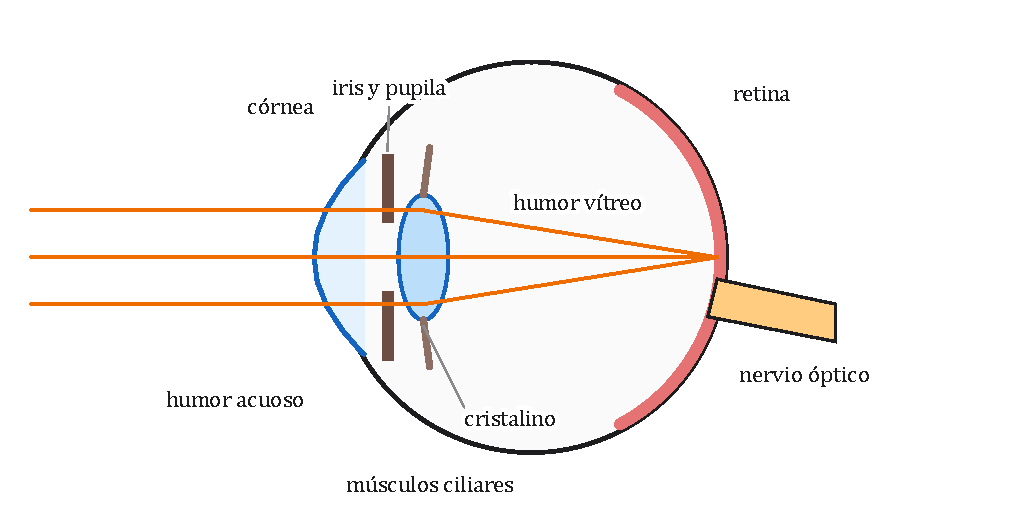
\includegraphics[width=0.66\linewidth]{images/UD3/ojo}
    \caption{Partes del ojo humano. La luz de un objeto lejano converge sobre la retina.}
    \label{fig:opt-ojo}
\end{figure}

\paragraph{Acomodación.} La distancia entre el cristalino y la retina es fija, así que para enfocar objetos a distintas
distancias el ojo cambia la curvatura del cristalino con los \emph{músculos ciliares}: es la \azuln{acomodación}. El punto
más lejano que se ve nítido sin esfuerzo es el \azuln{punto remoto} (el infinito para un ojo normal), y el más cercano, el
\azuln{punto próximo} (unos \qty{25}{\cm} en un adulto joven; unos \qty{7}{\cm} en un niño y hasta \qty{2}{\m} en una persona
mayor).

\subsection{Defectos de la visión}\label{subsec:opt-defectos}

\begin{itemize}
    \item \textbf{Miopía}. El ojo es demasiado convergente (o demasiado largo): la imagen de los objetos lejanos se forma
    \emph{delante} de la retina y se ven borrosos. Se corrige con \textbf{lentes divergentes}, cuyo foco imagen coincide con
    el punto remoto del ojo, o con cirugía láser de la córnea.
    \item \textbf{Hipermetropía}. El ojo es poco convergente: la imagen de los objetos cercanos se formaría \emph{detrás} de
    la retina. El punto próximo está más lejos de lo normal. Se corrige con \textbf{lentes convergentes}.
    \item \textbf{Presbicia} o vista cansada. Con la edad el cristalino pierde flexibilidad, la acomodación disminuye y el
    punto próximo se aleja. Se corrige con lentes convergentes para ver de cerca.
    \item \textbf{Astigmatismo}. La córnea no es perfectamente esférica y el ojo no enfoca a la vez las líneas verticales y
    las horizontales. Se corrige con lentes cilíndricas.
\end{itemize}

\begin{figure}[H]
    \centering
    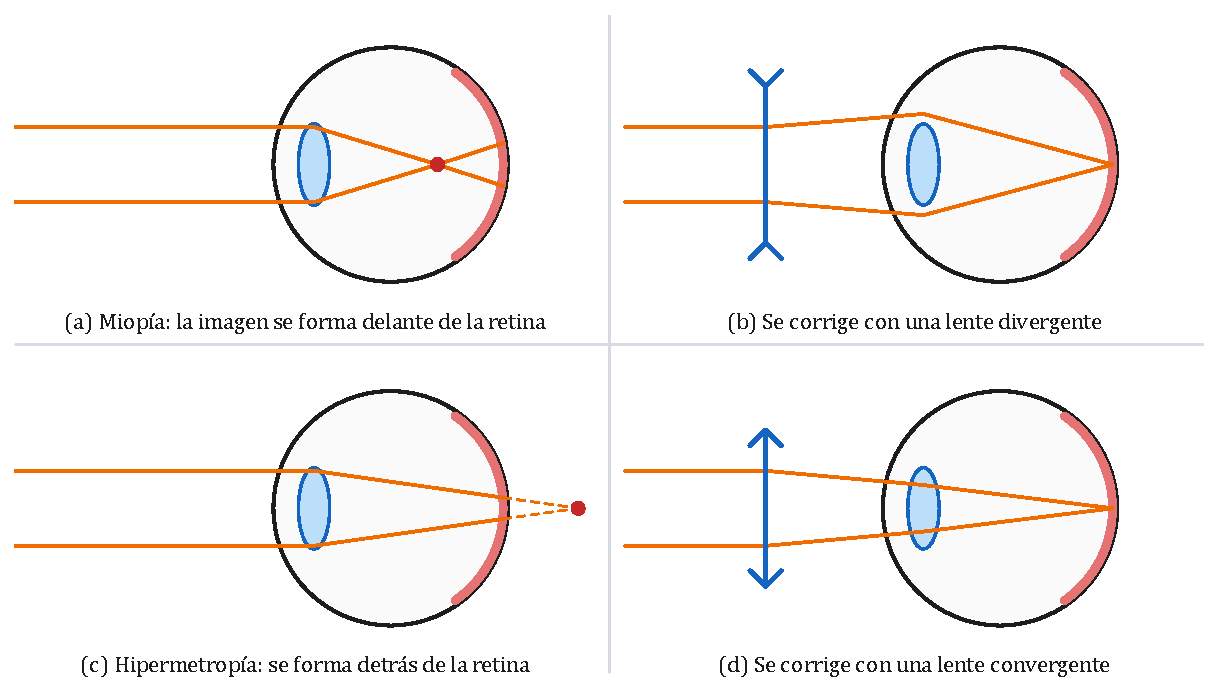
\includegraphics[width=0.9\linewidth]{images/UD3/defectos_vision}
    \caption{Miopía e hipermetropía y su corrección.}
    \label{fig:opt-defectos}
\end{figure}

\begin{exercise}
    El punto remoto de una persona miope está a \qty{50}{\cm}. ¿Qué lente necesita para ver bien de lejos?
    \begin{solu}
        \textcolor{blue}{La lente debe formar la imagen de un objeto en el infinito en el punto remoto: \(s = -\infty\), \(s' = \qty{-50}{\cm}\).}
        \(\dfrac{1}{f'} = \dfrac{1}{-50} - 0 \Rightarrow f' = \qty{-50}{\cm}\):
        \textcolor{red}{divergente de \(P = \dfrac{1}{-0{,}5} = \qty{-2}{D}\)}.
    \end{solu}
\end{exercise}

\begin{exercise}
    Una persona hipermétrope tiene el punto próximo a \qty{75}{\cm}. ¿Qué lente necesita para leer a \qty{25}{\cm}?
    \begin{solu}
        \textcolor{blue}{La lente debe dar, de un texto a \(s = \qty{-25}{\cm}\), una imagen virtual en su punto próximo, \(s' = \qty{-75}{\cm}\):}
        \(\dfrac{1}{f'} = \dfrac{1}{-75} - \dfrac{1}{-25} = \dfrac{2}{75} \Rightarrow f' = \qty{37.5}{\cm}\):
        \textcolor{red}{convergente de \(P = \qty{2.67}{D}\)}.
    \end{solu}
\end{exercise}

\section{Instrumentos ópticos}\label{sec:opt-instrumentos}

\subsection{La lupa}\label{subsec:opt-lupa}

Para ver un objeto con detalle lo acercamos al ojo: así ocupa un ángulo mayor y su imagen en la retina es más grande. Pero
no podemos acercarlo más que el punto próximo. La \rojon{lupa} es una lente convergente de distancia focal corta: si se pone
el objeto \textbf{entre el foco y la lente}, da una imagen \textbf{virtual, derecha y mayor} (figura~\ref{fig:opt-lupa}). Si
el objeto se coloca justo en el foco, la imagen está en el infinito y se ve sin necesidad de acomodar. El aumento de una
lupa en ese caso es aproximadamente \(M = \dfrac{\qty{0.25}{\m}}{f'}\).

\begin{figure}[H]
    \centering
    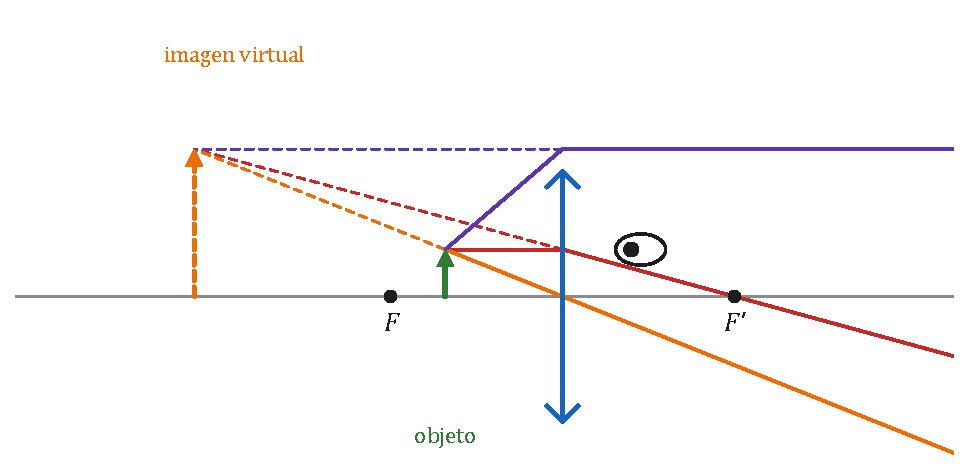
\includegraphics[width=0.62\linewidth]{images/UD3/lupa}
    \caption{Con el objeto dentro de la distancia focal, la lupa da una imagen virtual y aumentada.}
    \label{fig:opt-lupa}
\end{figure}

\begin{exercise}
    Queremos observar un mosquito con una lupa de \qty{4}{\cm} de distancia focal y ver su imagen 15 veces mayor. ¿A qué
    distancia de la lupa hay que ponerlo?
    \begin{solu}
        \textcolor{blue}{Imagen derecha: \(\beta = \dfrac{s'}{s} = 15 \Rightarrow s' = 15s\). En la ecuación de las lentes:}
        \[ \dfrac{1}{15s} - \dfrac{1}{s} = \dfrac{1}{4} \;\Rightarrow\; \dfrac{-14}{15s} = \dfrac{1}{4} \;\Rightarrow\; \textcolor{red}{s = \qty{-3.73}{\cm}} \]
        \textcolor{blue}{A \qty{3.73}{\cm} de la lupa, dentro de la distancia focal; la imagen está en \(s' = \qty{-56}{\cm}\).}
    \end{solu}
\end{exercise}

\subsection{El microscopio}\label{subsec:opt-microscopio}

El \rojon{microscopio} tiene dos lentes convergentes de distancia focal pequeña (figura~\ref{fig:opt-microscopio}):
\begin{itemize}
    \item El \textbf{objetivo}, la lente cercana al objeto. El objeto se coloca un poco más allá de su foco y el objetivo
    da una imagen \(y'_1\) \textbf{real, invertida y mucho mayor}.
    \item El \textbf{ocular}, la lente por la que se mira. La imagen \(y'_1\) queda entre el ocular y su foco objeto, y el
    ocular actúa como una lupa: da una imagen final \(y'_2\) \textbf{virtual} y mucho mayor (invertida respecto del objeto).
\end{itemize}
El aumento total es el producto de los aumentos del objetivo y del ocular: un objetivo \(40\times\) con un ocular
\(10\times\) aumenta \(400\) veces.

\begin{figure}[H]
    \centering
    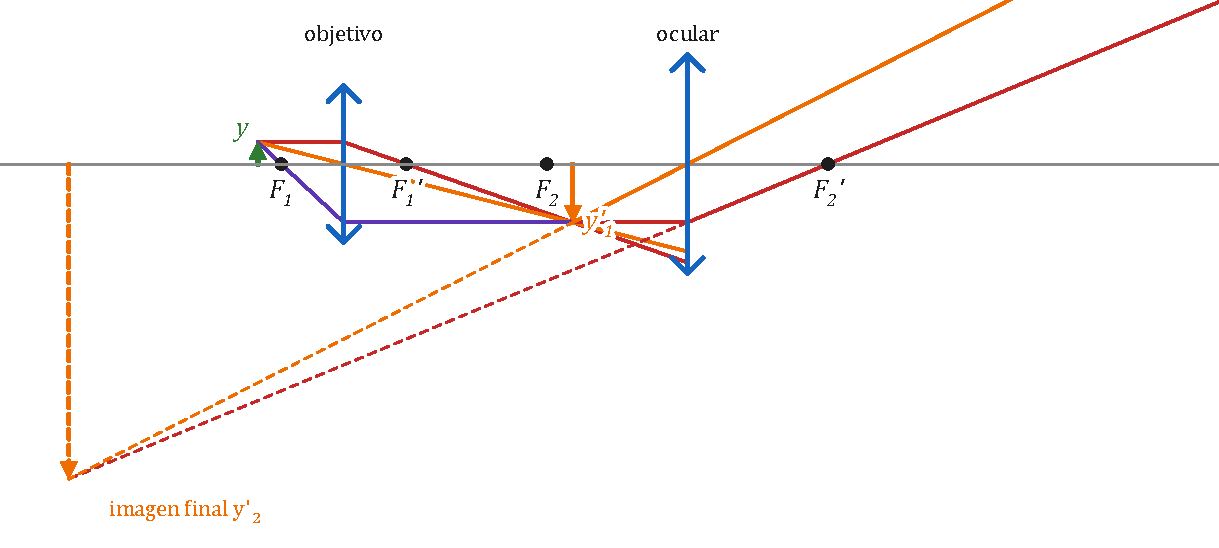
\includegraphics[width=0.9\linewidth]{images/UD3/microscopio}
    \caption{Formación de la imagen en un microscopio.}
    \label{fig:opt-microscopio}
\end{figure}

\section{Resumen de fórmulas}\label{sec:opt-resumen}

\begin{table}[H]
    \centering
    \caption{Fórmulas principales de la óptica geométrica (convenio DIN)}
    \vspace{-5pt}
    \begin{tabular}{@{}lL{10cm}@{}}
        \toprule
        \textbf{Magnitud} & \textbf{Expresión} \\
        \midrule
        Índice de refracción & \(n = c/v\), \quad \(\lambda = \lambda_0/n\) \\[3pt]
        Ley de Snell & \(n_1\sen\hat{\imath} = n_2\sen\hat r\) \\[3pt]
        Ángulo límite & \(\sen\hat{\imath}_L = n_2/n_1\) \quad (\(n_1 > n_2\)) \\[3pt]
        Lámina de caras paralelas & \(\delta = e\sen(\hat{\imath} - \hat r)/\cos\hat r\) \\[3pt]
        Prisma & \(\varphi = \hat r_1 + \hat{\imath}_2\), \quad \(\delta = \hat{\imath}_1 + \hat r_2 - \varphi\) \\[3pt]
        Desviación mínima & \(n = \sen\frac{\delta_m + \varphi}{2}\big/\sen\frac{\varphi}{2}\) \\[3pt]
        Dioptrio esférico & \(n'/s' - n/s = (n' - n)/R\), \quad \(\beta = n s'/(n' s)\) \\[3pt]
        Focales del dioptrio & \(f' = R\,n'/(n' - n)\), \quad \(f = -R\,n/(n' - n)\) \\[3pt]
        Dioptrio plano & \(s'/s = n'/n\), \quad \(\beta = 1\) \\[3pt]
        Espejos & \(1/s' + 1/s = 1/f\), \quad \(f = R/2\), \quad \(\beta = -s'/s\) \\[3pt]
        Lentes delgadas & \(1/s' - 1/s = 1/f'\), \quad \(\beta = s'/s\), \quad \(P = 1/f'\) \\[3pt]
        Constructor de lentes & \(1/f' = (n - 1)(1/R_1 - 1/R_2)\) \\
        \bottomrule
    \end{tabular}
    \label{tab:opt-resumen}
\end{table}

\section{Prácticas de laboratorio}\label{sec:opt-practicas}

\subsection{Práctica 1: ley de Snell y ángulo límite}\label{subsec:opt-practica-snell}

\noindent\begin{minipage}[t]{0.6\linewidth}
\textbf{Objetivo.} Comprobar la ley de Snell, medir el índice de refracción de un bloque de metacrilato y observar la
reflexión total.

\textbf{Material.} Disco graduado (goniómetro), bloque semicircular de metacrilato o vidrio, puntero láser o lámpara con
rendija.

\textbf{Procedimiento.}
\begin{enumerate}[label=\numberballmDarkTeal]
    \item Coloca el semicilindro sobre el disco con la cara plana en el diámetro y su centro en el centro del disco
    (figura~\ref{fig:opt-practica-snell}).
    \item Haz llegar el láser al centro de la cara plana con distintos ángulos de incidencia y anota los ángulos de
    refracción. El rayo sale por la cara curva sin desviarse, porque la cruza perpendicularmente.
    \item Gira el disco para que la luz entre por la cara curva y salga por la plana. Aumenta el ángulo hasta que el rayo
    refractado desaparezca y mide el ángulo límite.
\end{enumerate}
\end{minipage}\hfill
\begin{minipage}[t]{0.36\linewidth}
    \vspace{0pt}
    \centering
    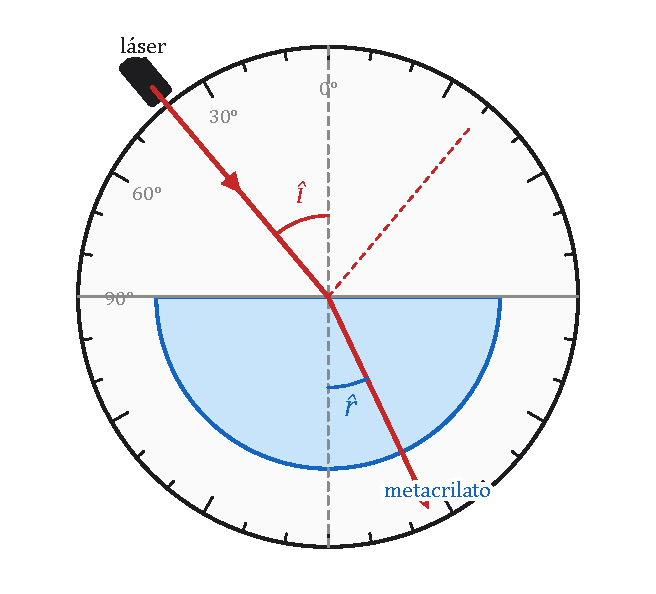
\includegraphics[width=\linewidth]{images/UD3/practica_snell}
    \captionof{figure}{Medida de los ángulos.}
    \label{fig:opt-practica-snell}
\end{minipage}

\begin{table}[H]
    \centering
    \caption{Datos de la práctica de la ley de Snell}
    \vspace{-5pt}
    \begin{tabular}{@{}C{2.4cm}C{2.4cm}C{2.4cm}C{2.4cm}C{2.6cm}@{}}
        \toprule
        \textbf{\(\hat{\imath}\) (\unit{\degree})} & \textbf{\(\hat r\) (\unit{\degree})} & \textbf{\(\sen\hat{\imath}\)} & \textbf{\(\sen\hat r\)} & \textbf{\(n = \sen\hat{\imath}/\sen\hat r\)} \\
        \midrule
        \rule{0pt}{18pt} & & & & \\ \midrule[0.3pt]
        \rule{0pt}{18pt} & & & & \\ \midrule[0.3pt]
        \rule{0pt}{18pt} & & & & \\ \midrule[0.3pt]
        \rule{0pt}{18pt} & & & & \\
        \bottomrule
    \end{tabular}
    \label{tab:opt-practica-snell}
\end{table}

\textbf{Cálculos.} Representa \(\sen\hat{\imath}\) frente a \(\sen\hat r\): debe salir una recta que pasa por el origen y
cuya pendiente es \(n\).

\textbf{Cuestiones.}
\begin{enumerate}[label=\letraminuscula]
    \item Con el índice obtenido, calcula el ángulo límite teórico y compáralo con el medido.
    \item ¿Por qué hay que hacer llegar el rayo al centro de la cara plana?
    \item ¿Qué observas en el rayo reflejado a medida que te acercas al ángulo límite?
\end{enumerate}

\subsection{Práctica 2: distancia focal de una lente convergente}\label{subsec:opt-practica-lente}

\textbf{Objetivo.} Medir la distancia focal de una lente convergente con el banco óptico y comprobar la ecuación de las
lentes.

\textbf{Material.} Banco óptico con regla, lámpara, objeto (una flecha o una letra recortada en una cartulina), lente
convergente con soporte y pantalla.

\begin{figure}[H]
    \centering
    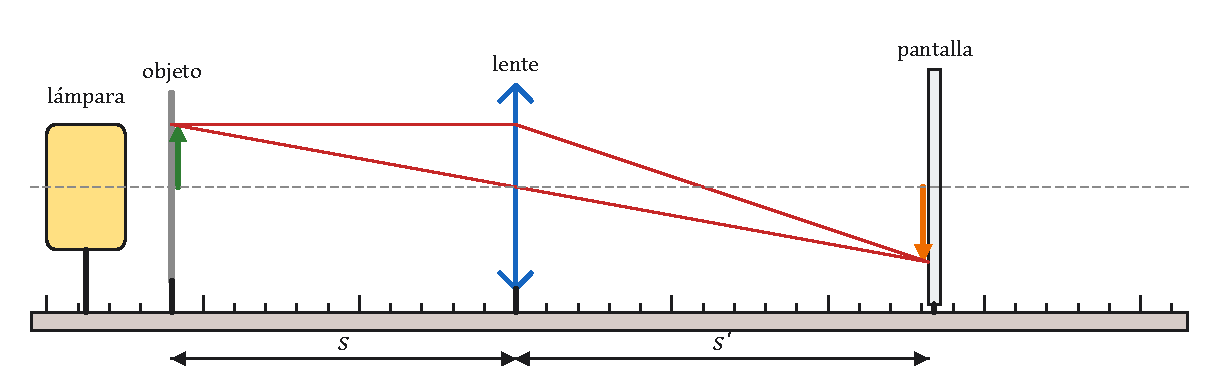
\includegraphics[width=0.85\linewidth]{images/UD3/practica_lente}
    \caption{Montaje en el banco óptico. Se mueve la pantalla hasta que la imagen se ve nítida.}
    \label{fig:opt-practica-lente}
\end{figure}

\textbf{Procedimiento.}
\begin{enumerate}[label=\numberballmDarkTeal]
    \item Estimación rápida: enfoca con la lente la imagen de una ventana lejana sobre una pared. La distancia de la lente
    a la pared es, aproximadamente, \(f'\).
    \item Monta el banco (figura~\ref{fig:opt-practica-lente}). Coloca el objeto a una distancia \(|s|\) mayor que \(f'\) y
    mueve la pantalla hasta ver la imagen nítida. Mide \(s\), \(s'\) y el tamaño de la imagen.
    \item Repite para al menos cuatro distancias distintas.
\end{enumerate}

\begin{table}[H]
    \centering
    \caption{Datos de la práctica de la lente convergente}
    \vspace{-5pt}
    \begin{tabular}{@{}C{2.2cm}C{2.2cm}C{2.4cm}C{2.4cm}C{2.4cm}C{2cm}@{}}
        \toprule
        \textbf{\(s\) (\unit{\cm})} & \textbf{\(s'\) (\unit{\cm})} & \textbf{\(1/s\) (\unit{\per\cm})} & \textbf{\(1/s'\) (\unit{\per\cm})} & \textbf{\(f'\) (\unit{\cm})} & \textbf{\(\beta\)} \\
        \midrule
        \rule{0pt}{18pt} & & & & & \\ \midrule[0.3pt]
        \rule{0pt}{18pt} & & & & & \\ \midrule[0.3pt]
        \rule{0pt}{18pt} & & & & & \\ \midrule[0.3pt]
        \rule{0pt}{18pt} & & & & & \\
        \bottomrule
    \end{tabular}
    \label{tab:opt-practica-lente}
\end{table}

\textbf{Cálculos.} Con cada pareja calcula \(f'\) con \(1/f' = 1/s' - 1/s\) (recuerda que \(s < 0\)) y halla la media.
Método gráfico: representa \(1/s'\) frente a \(1/s\); es una recta de pendiente 1 cuya ordenada en el origen es \(1/f'\).

\textbf{Cuestiones.}
\begin{enumerate}[label=\letraminuscula]
    \item Compara el aumento medido (\(y'/y\)) con el calculado (\(s'/s\)).
    \item ¿Qué pasa si colocas el objeto entre el foco y la lente? ¿Puedes recoger la imagen en la pantalla? ¿Por qué?
    \item Calcula la potencia de la lente en dioptrías.
\end{enumerate}
